
\documentclass[11pt,a4paper]{article}

\usepackage[utf8]{inputenc}
\usepackage[T1]{fontenc}
\usepackage[spanish,es-noshorthands]{babel}
\usepackage{lmodern}
\usepackage{geometry}
\usepackage{graphicx}
\usepackage{booktabs}
\usepackage{array}
\usepackage{float}
\usepackage{amsmath}
\usepackage{xcolor}
\usepackage{fancyhdr}
\usepackage{microtype}
\usepackage{hyperref}

\geometry{margin=2.5cm}
\graphicspath{{../../results/figures/students/}}
\definecolor{azulacademico}{RGB}{20,53,91}

\hypersetup{
    colorlinks=true,
    linkcolor=azulacademico,
    urlcolor=azulacademico,
    citecolor=azulacademico
}

\pagestyle{fancy}
\fancyhf{}
\fancyhead[L]{Proyecto 9 -- Inteligencia Artificial}
\fancyhead[R]{Yachay Tech}
\fancyfoot[C]{\thepage}
\setlength{\headheight}{14pt}
\setlength{\parskip}{5pt}

\begin{document}

% ======================================
% PORTADA
% ======================================

\begin{titlepage}
\centering
\vspace*{2.5cm}

{\Large\bfseries UNIVERSIDAD YACHAY TECH\par}
\vspace{0.4cm}
{\large Maestría en Ciencia de Datos\par}
{\large Fundamentos de Inteligencia Artificial\par}

\vspace{2.5cm}

{\Huge\bfseries Predicción del estado académico universitario\par}

\vspace{0.7cm}

{\LARGE Redes neuronales multicategoría,
optimización con Optuna y análisis de interpretabilidad\par}

\vspace{2cm}

{\large\textbf{Autor:}\par}
{\large Héctor Alexander Román Potosí\par}

\vspace{0.8cm}

{\large\textbf{Docente:}\par}
{\large PhD. Eugenio Morocho\par}

\vfill
{\large Noviembre de 2026\par}
{\large Ecuador\par}

\end{titlepage}

% ======================================
% RESUMEN
% ======================================

\begin{abstract}
Este trabajo estudia la predicción del estado académico
universitario mediante redes neuronales artificiales.
Se empleó el conjunto de datos UCI 697, compuesto por
4424 estudiantes, 36 variables predictoras y tres clases:
abandono, permanencia y graduación.

Se diseñaron cuatro escenarios de disponibilidad de
información, se entrenaron modelos base con Keras y
se realizaron 80 ensayos de optimización mediante
Optuna y el algoritmo TPE.

Además, se investigó el efecto del balanceo de clases
mediante nueve entrenamientos adicionales.
El modelo principal, con balanceo moderado,
obtuvo un macro-F1 de 0,7107 en prueba.
Su recall para la clase Enrolled fue de 0,5220,
frente a 0,4403 del modelo Optuna sin balanceo.

El análisis bootstrap pareado no proporcionó
evidencia concluyente de mejora global en macro-F1,
aunque el intervalo para la diferencia en recall de
Enrolled fue positivo.
La importancia por permutación destacó el rendimiento
académico del segundo semestre como información predictiva
especialmente relevante.

Los resultados muestran la utilidad de la optimización y
del análisis de desbalance, así como la necesidad de
evaluar las compensaciones entre clases.
\end{abstract}

\noindent\textbf{Palabras clave:}
redes neuronales, clasificación multiclase,
Optuna, macro-F1, deserción universitaria,
interpretabilidad.

\tableofcontents
\clearpage

% ======================================
\section{Introducción}
% ======================================

La predicción de resultados académicos constituye
un problema de clasificación supervisada con
aplicaciones potenciales en el análisis educativo.

Este estudio investiga tres posibles resultados:
\texttt{Dropout}, \texttt{Enrolled} y
\texttt{Graduate}.

El propósito no es tomar decisiones individuales
automáticas sobre estudiantes, sino comparar
metodologías de aprendizaje automático y
comprender sus limitaciones.

Se utiliza el conjunto de datos
\emph{Predict Students' Dropout and Academic Success},
publicado en el repositorio UCI \cite{uci697}.

\subsection{Pregunta de investigación}

¿En qué medida la información académica disponible,
la optimización de hiperparámetros y el balanceo
de clases modifican el rendimiento de una red neuronal
para clasificación multiclase?

\subsection{Objetivos}

El objetivo general consiste en desarrollar y
evaluar modelos de redes neuronales para
clasificar el estado académico universitario.

Los objetivos específicos son:
\begin{enumerate}
\item Preparar los datos mediante procedimientos reproducibles.
\item Comparar cuatro escenarios de variables predictoras.
\item Optimizar redes neuronales con Optuna.
\item Analizar el efecto del desbalance de clases.
\item Evaluar la generalización sobre datos reservados.
\item Examinar la importancia predictiva de las variables.
\end{enumerate}

% ======================================
\section{Conjunto de datos}
% ======================================

El dataset contiene 4424 observaciones y
36 variables predictoras.
No se identificaron valores faltantes ni
duplicados exactos en la auditoría realizada.

\begin{table}[H]
\centering
\caption{Distribución de las clases}
\begin{tabular}{lrr}
\toprule
Clase & Registros & Porcentaje \\
\midrule
Dropout & 1421 & 32,12 \% \\
Enrolled & 794 & 17,95 \% \\
Graduate & 2209 & 49,93 \% \\
\bottomrule
\end{tabular}
\end{table}

La distribución evidencia un desbalance:
la clase Enrolled tiene considerablemente
menos observaciones que Graduate.

\begin{figure}[H]
\centering
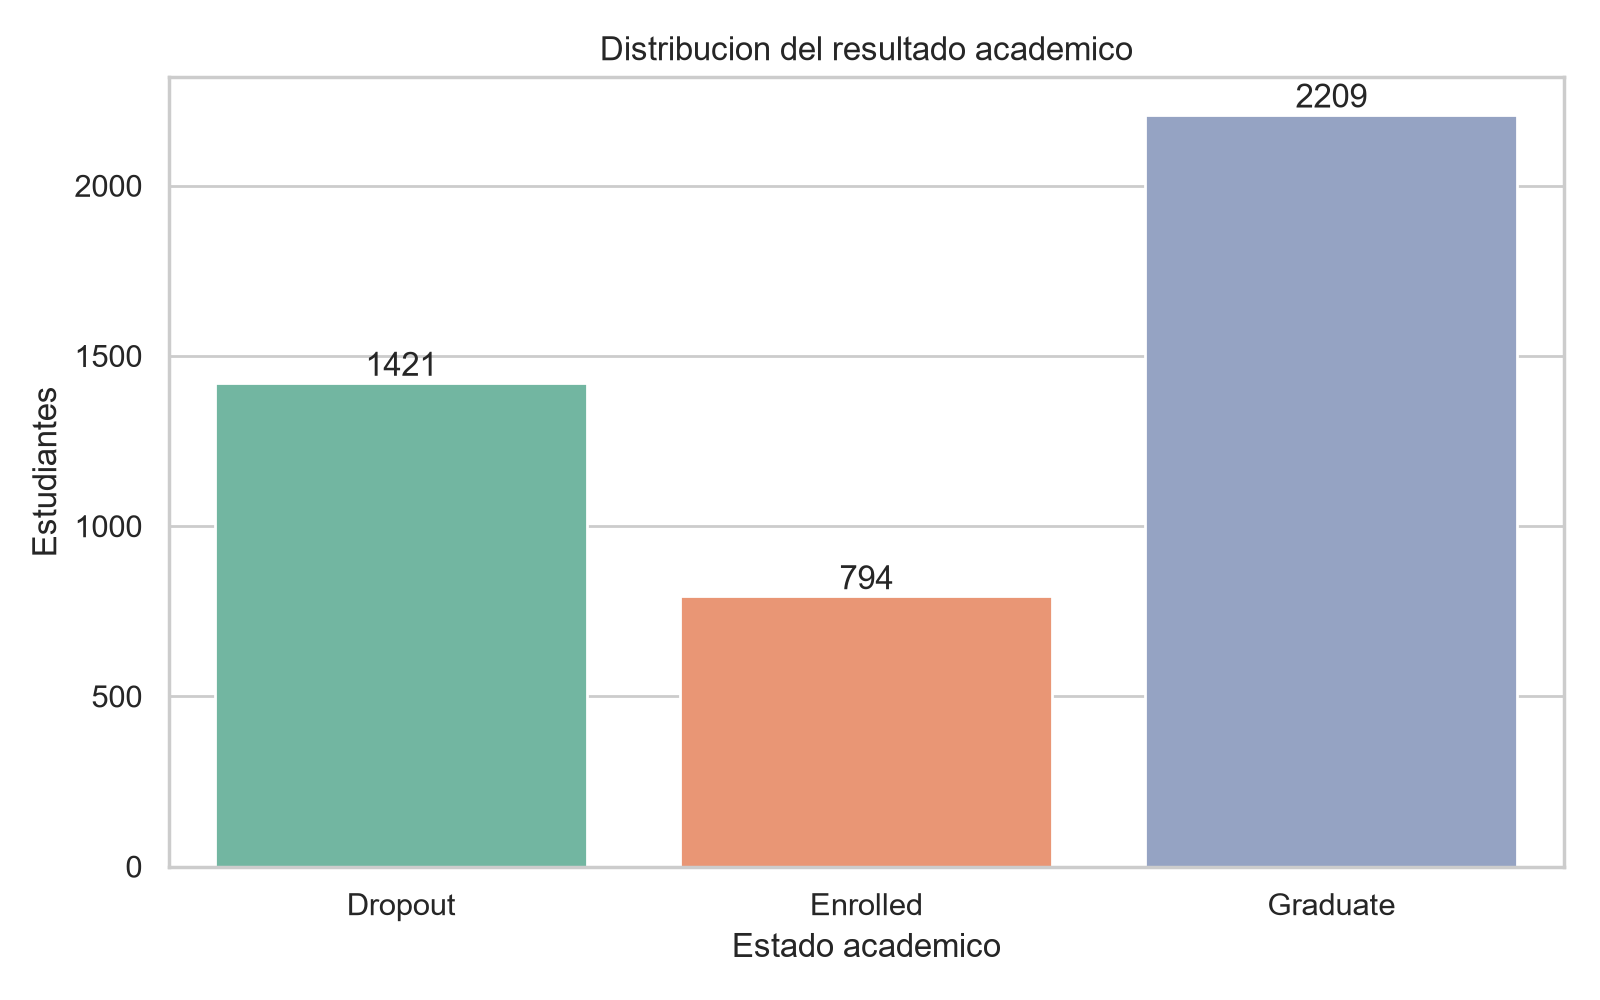
\includegraphics[width=0.82\linewidth]{01_clases.png}
\caption{Distribución de clases en el conjunto de datos.}
\end{figure}

\subsection{Escenarios de información}

Se definieron cuatro escenarios:
\begin{table}[H]
\centering
\caption{Escenarios de clasificación}
\begin{tabular}{lrr}
\toprule
Escenario & Variables originales & Codificadas \\
\midrule
A: Sin semestres & 21 & 206 \\
B: Primer semestre & 27 & 212 \\
C: Dos semestres & 33 & 218 \\
D: Completo & 36 & 221 \\
\bottomrule
\end{tabular}
\end{table}

Los escenarios permiten investigar el
aporte incremental de información académica.

Algunas variables financieras y administrativas
pueden actualizarse durante la trayectoria
universitaria. Por ello, el escenario A no debe
interpretarse automáticamente como una predicción
estrictamente realizada al ingreso.

% ======================================
\section{Metodología}
% ======================================

\subsection{División y preprocesamiento}

Se utilizó una división estratificada:

\begin{itemize}
\item Entrenamiento: 2654 observaciones.
\item Validación: 885 observaciones.
\item Prueba: 885 observaciones.
\end{itemize}

Las variables nominales fueron transformadas
mediante One-Hot Encoding.
Las variables cuantitativas se estandarizaron
mediante StandardScaler.

Los transformadores se ajustaron exclusivamente
con entrenamiento para evitar fugas de información.

Los cuatro escenarios compartieron las mismas
observaciones en cada partición.

\subsection{Modelo neuronal de referencia}

La arquitectura base contiene dos capas ocultas
de 12 y 8 neuronas con activación ReLU.
La capa final utiliza tres neuronas con softmax.

Para cada clase $k$, la salida se define mediante:
\[
p_k =
\frac{\exp(z_k)}
{\sum_{j=1}^{3}\exp(z_j)}.
\]

Se empleó Adam y la función
\texttt{sparse\_categorical\_crossentropy}.

El entrenamiento incorporó Early Stopping.

\subsection{Optimización con Optuna}

Se utilizó TPESampler para maximizar el macro-F1
de validación.

Se exploraron:
\begin{itemize}
\item Número de capas ocultas: de 1 a 3.
\item Neuronas: 16, 32, 64 o 128 por capa.
\item Dropout: de 0 a 0,4.
\item Regularización L2: de $10^{-6}$ a $10^{-3}$.
\item Learning rate: de $10^{-4}$ a $5\times10^{-3}$.
\item Tamaños de lote: 16, 32 y 64.
\end{itemize}

Se completaron 20 ensayos por escenario,
para un total de 80 ensayos.

\subsection{Métricas}

Se utilizaron accuracy, balanced accuracy,
recall por clase y macro-F1.

El macro-F1 se define como:
\[
F_{1,\mathrm{macro}} =
\frac{1}{3}\sum_{k=1}^{3}F_{1,k},
\]
donde
\[
F_{1,k} =
\frac{2P_kR_k}{P_k+R_k}.
\]

Esta métrica permite considerar por igual
las tres clases, independientemente de
sus frecuencias.

% ======================================
\section{Resultados de optimización}
% ======================================

\subsection{Resultados de validación}

\begin{table}[H]
\centering
\caption{Macro-F1 de validación}
\begin{tabular}{lrrr}
\toprule
Escenario & Base & Optuna & Mejora (pp) \\
\midrule
A & 0,4789 & 0,5627 & 8,38 \\
B & 0,6570 & 0,6857 & 2,87 \\
C & 0,6892 & 0,7142 & 2,50 \\
D & 0,7215 & 0,7219 & 0,03 \\
\bottomrule
\end{tabular}
\end{table}

La mayor mejora se observó en el escenario A.
En D, la diferencia fue prácticamente nula.

Esto indica que la optimización puede resultar
útil, pero su beneficio depende del escenario
y de la arquitectura de referencia.

\begin{figure}[H]
\centering
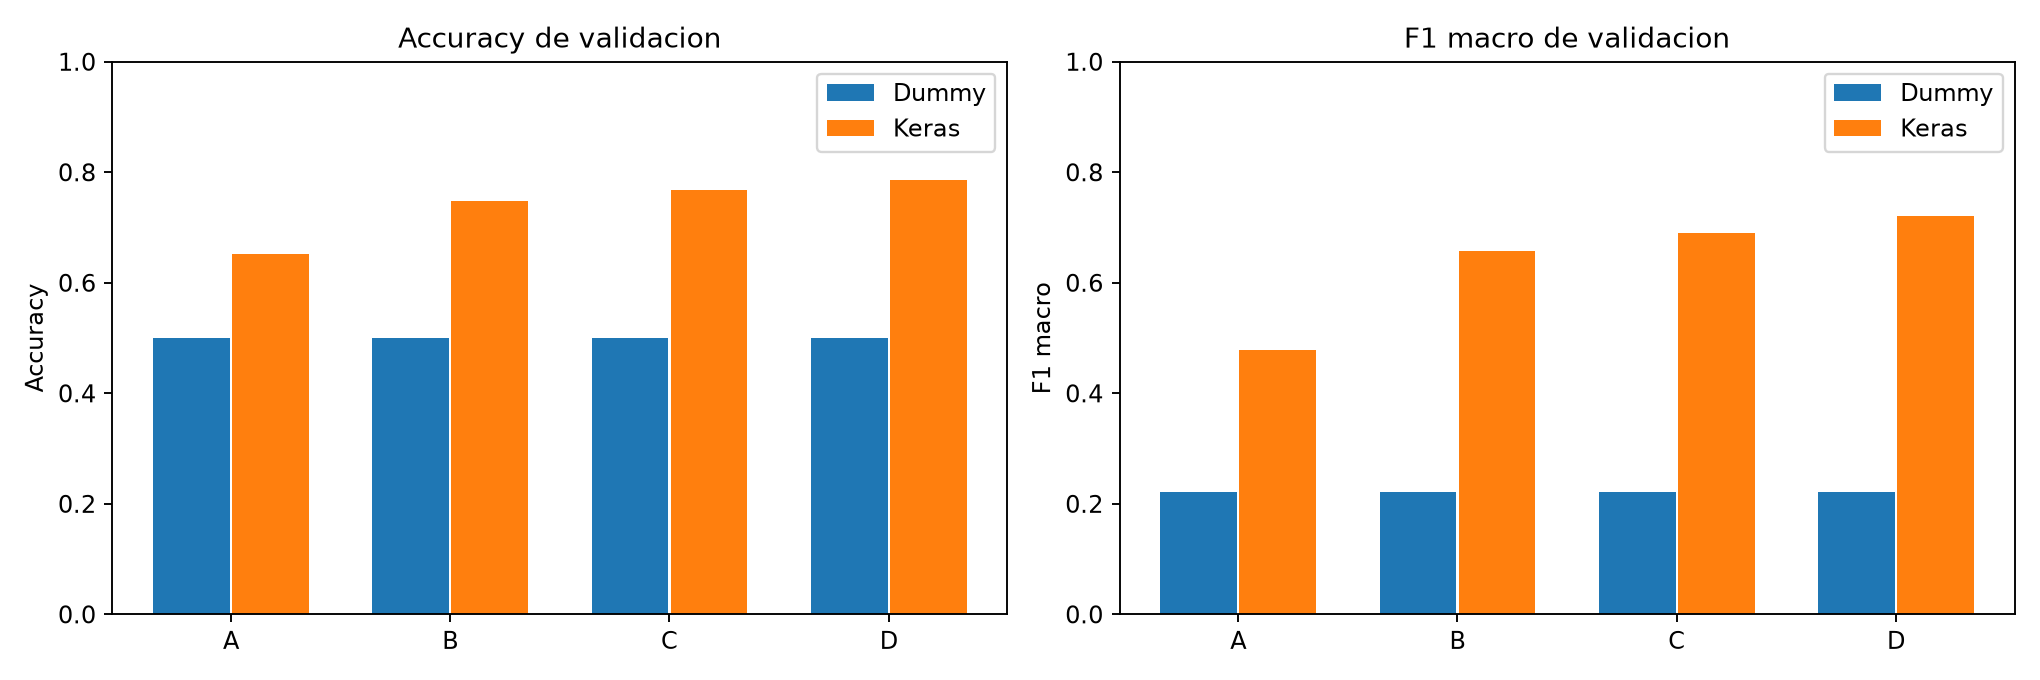
\includegraphics[width=0.85\linewidth]
{comparacion_baselines_validacion.png}
\caption{Rendimiento de las redes neuronales base en validación.}
\end{figure}

% ======================================
\section{Experimento de balanceo}
% ======================================

Se evaluaron tres estrategias en el escenario D:
sin pesos, balanceo moderado y balanceo completo.

Cada estrategia se entrenó con semillas
42, 123 y 2026.

\begin{table}[H]
\centering
\caption{Resultados promedio de validación}
\small
\begin{tabular}{lrrr}
\toprule
Estrategia & Macro-F1 & Recall Enrolled & Recall Dropout \\
\midrule
Sin pesos & 0,7099 & 0,3920 & 0,7899 \\
Moderado & 0,7259 & 0,4864 & 0,7887 \\
Balanceado & 0,7245 & 0,5765 & 0,7782 \\
\bottomrule
\end{tabular}
\end{table}

El balanceo completo favoreció el recall de
Enrolled, mientras que el moderado alcanzó
el mayor macro-F1 promedio.

Estas variaciones corresponden a entrenamientos
con diferentes semillas sobre una misma partición;
no equivalen a validación cruzada.

% ======================================
\section{Evaluación final independiente}
% ======================================

Se reservaron 885 observaciones para la
evaluación final, realizada después de cerrar
las decisiones de selección.

\begin{table}[H]
\centering
\caption{Comparación sobre el conjunto de prueba}
\small
\begin{tabular}{llrrr}
\toprule
Escenario & Modelo & Accuracy & Macro-F1 & Recall Enrolled \\
\midrule
A & Base & 0,6463 & 0,4647 & 0,0000 \\
A & Optuna & 0,6362 & 0,5059 & 0,1006 \\
B & Base & 0,7333 & 0,6335 & 0,2516 \\
B & Optuna & 0,7333 & 0,6486 & 0,3145 \\
C & Base & 0,7740 & 0,6968 & 0,3711 \\
C & Optuna & 0,7627 & 0,6887 & 0,3899 \\
D & Base & 0,7650 & 0,6896 & 0,3774 \\
D & Optuna & 0,7740 & 0,7097 & 0,4403 \\
D & Moderado & 0,7650 & 0,7107 & 0,5220 \\
D & Balanceado & 0,7469 & 0,7064 & 0,6164 \\
\bottomrule
\end{tabular}
\end{table}

\begin{figure}[H]
\centering
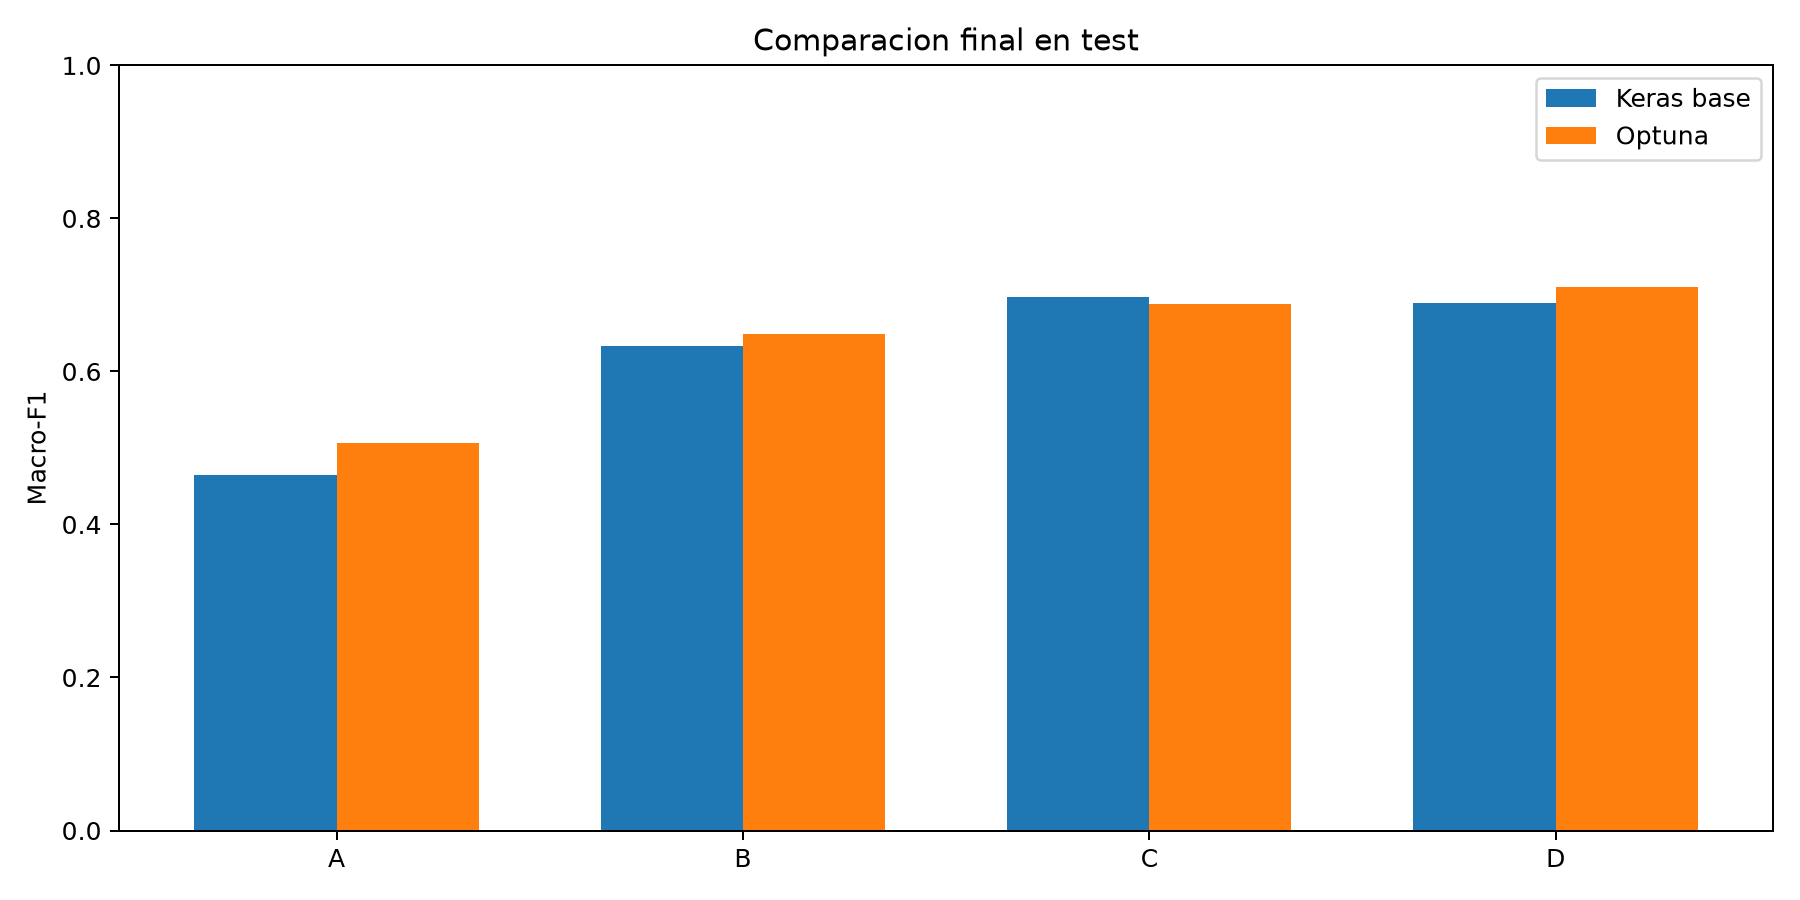
\includegraphics[width=0.88\linewidth]
{test_comparacion_escenarios.png}
\caption{Comparación del macro-F1 de los modelos base y Optuna en prueba.}
\end{figure}

El escenario D con balanceo moderado fue
seleccionado previamente como modelo principal.
Obtuvo macro-F1 de 0,7107 y recall Enrolled
de 0,5220 en prueba.

\begin{figure}[H]
\centering
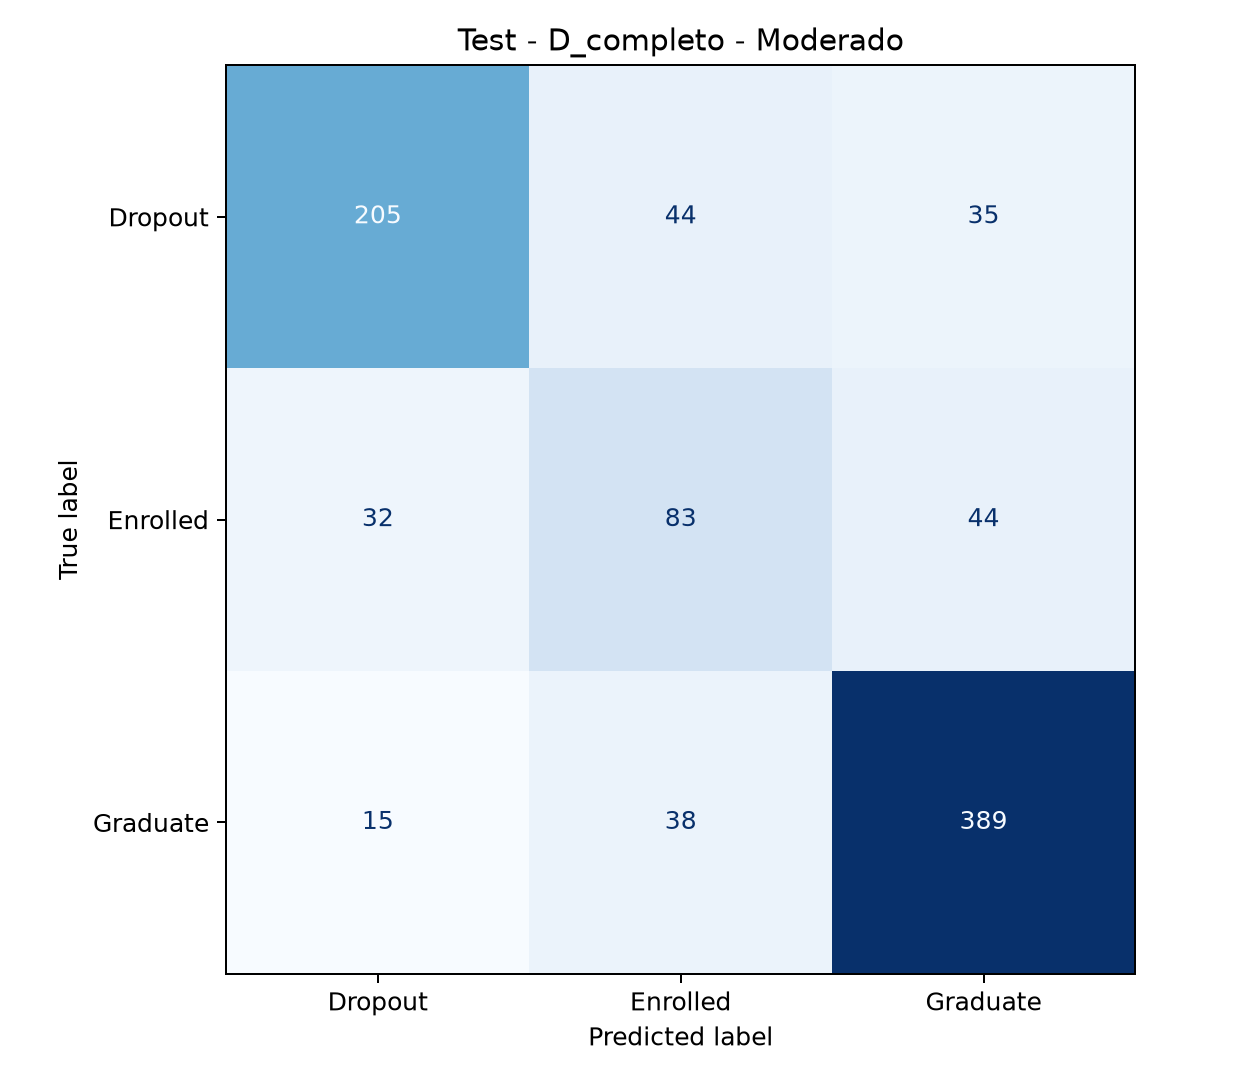
\includegraphics[width=0.75\linewidth]
{test_matriz_D_Moderado.png}
\caption{Matriz de confusión del modelo principal.}
\end{figure}

\subsection{Incertidumbre mediante bootstrap}

Se aplicó bootstrap pareado con
2000 remuestreos para comparar el modelo
D moderado frente a D Optuna.

Los intervalos percentiles del 95 \% fueron:
\[
\Delta F_{1,\mathrm{macro}}
\in [-0,0163,\;0,0191],
\]
\[
\Delta R_{\mathrm{Enrolled}}
\in [0,0427,\;0,1273].
\]

El primer intervalo incluye cero.
Por tanto, no se obtuvo evidencia concluyente
de una mejora global del macro-F1.

El segundo intervalo fue positivo,
lo que respalda una mejora del recall de Enrolled
en esta muestra de prueba.

Los intervalos están condicionados a esta
partición y a los modelos previamente fijados.

% ======================================
\section{Interpretabilidad}
% ======================================

Se realizó un análisis de importancia por
permutación sobre validación con el modelo
D de balanceo moderado.

La variable de mayor importancia fue
\texttt{Curricular units 2nd sem (approved)},
cuya permutación produjo una reducción media
de 0,14346 en macro-F1.

\begin{figure}[H]
\centering
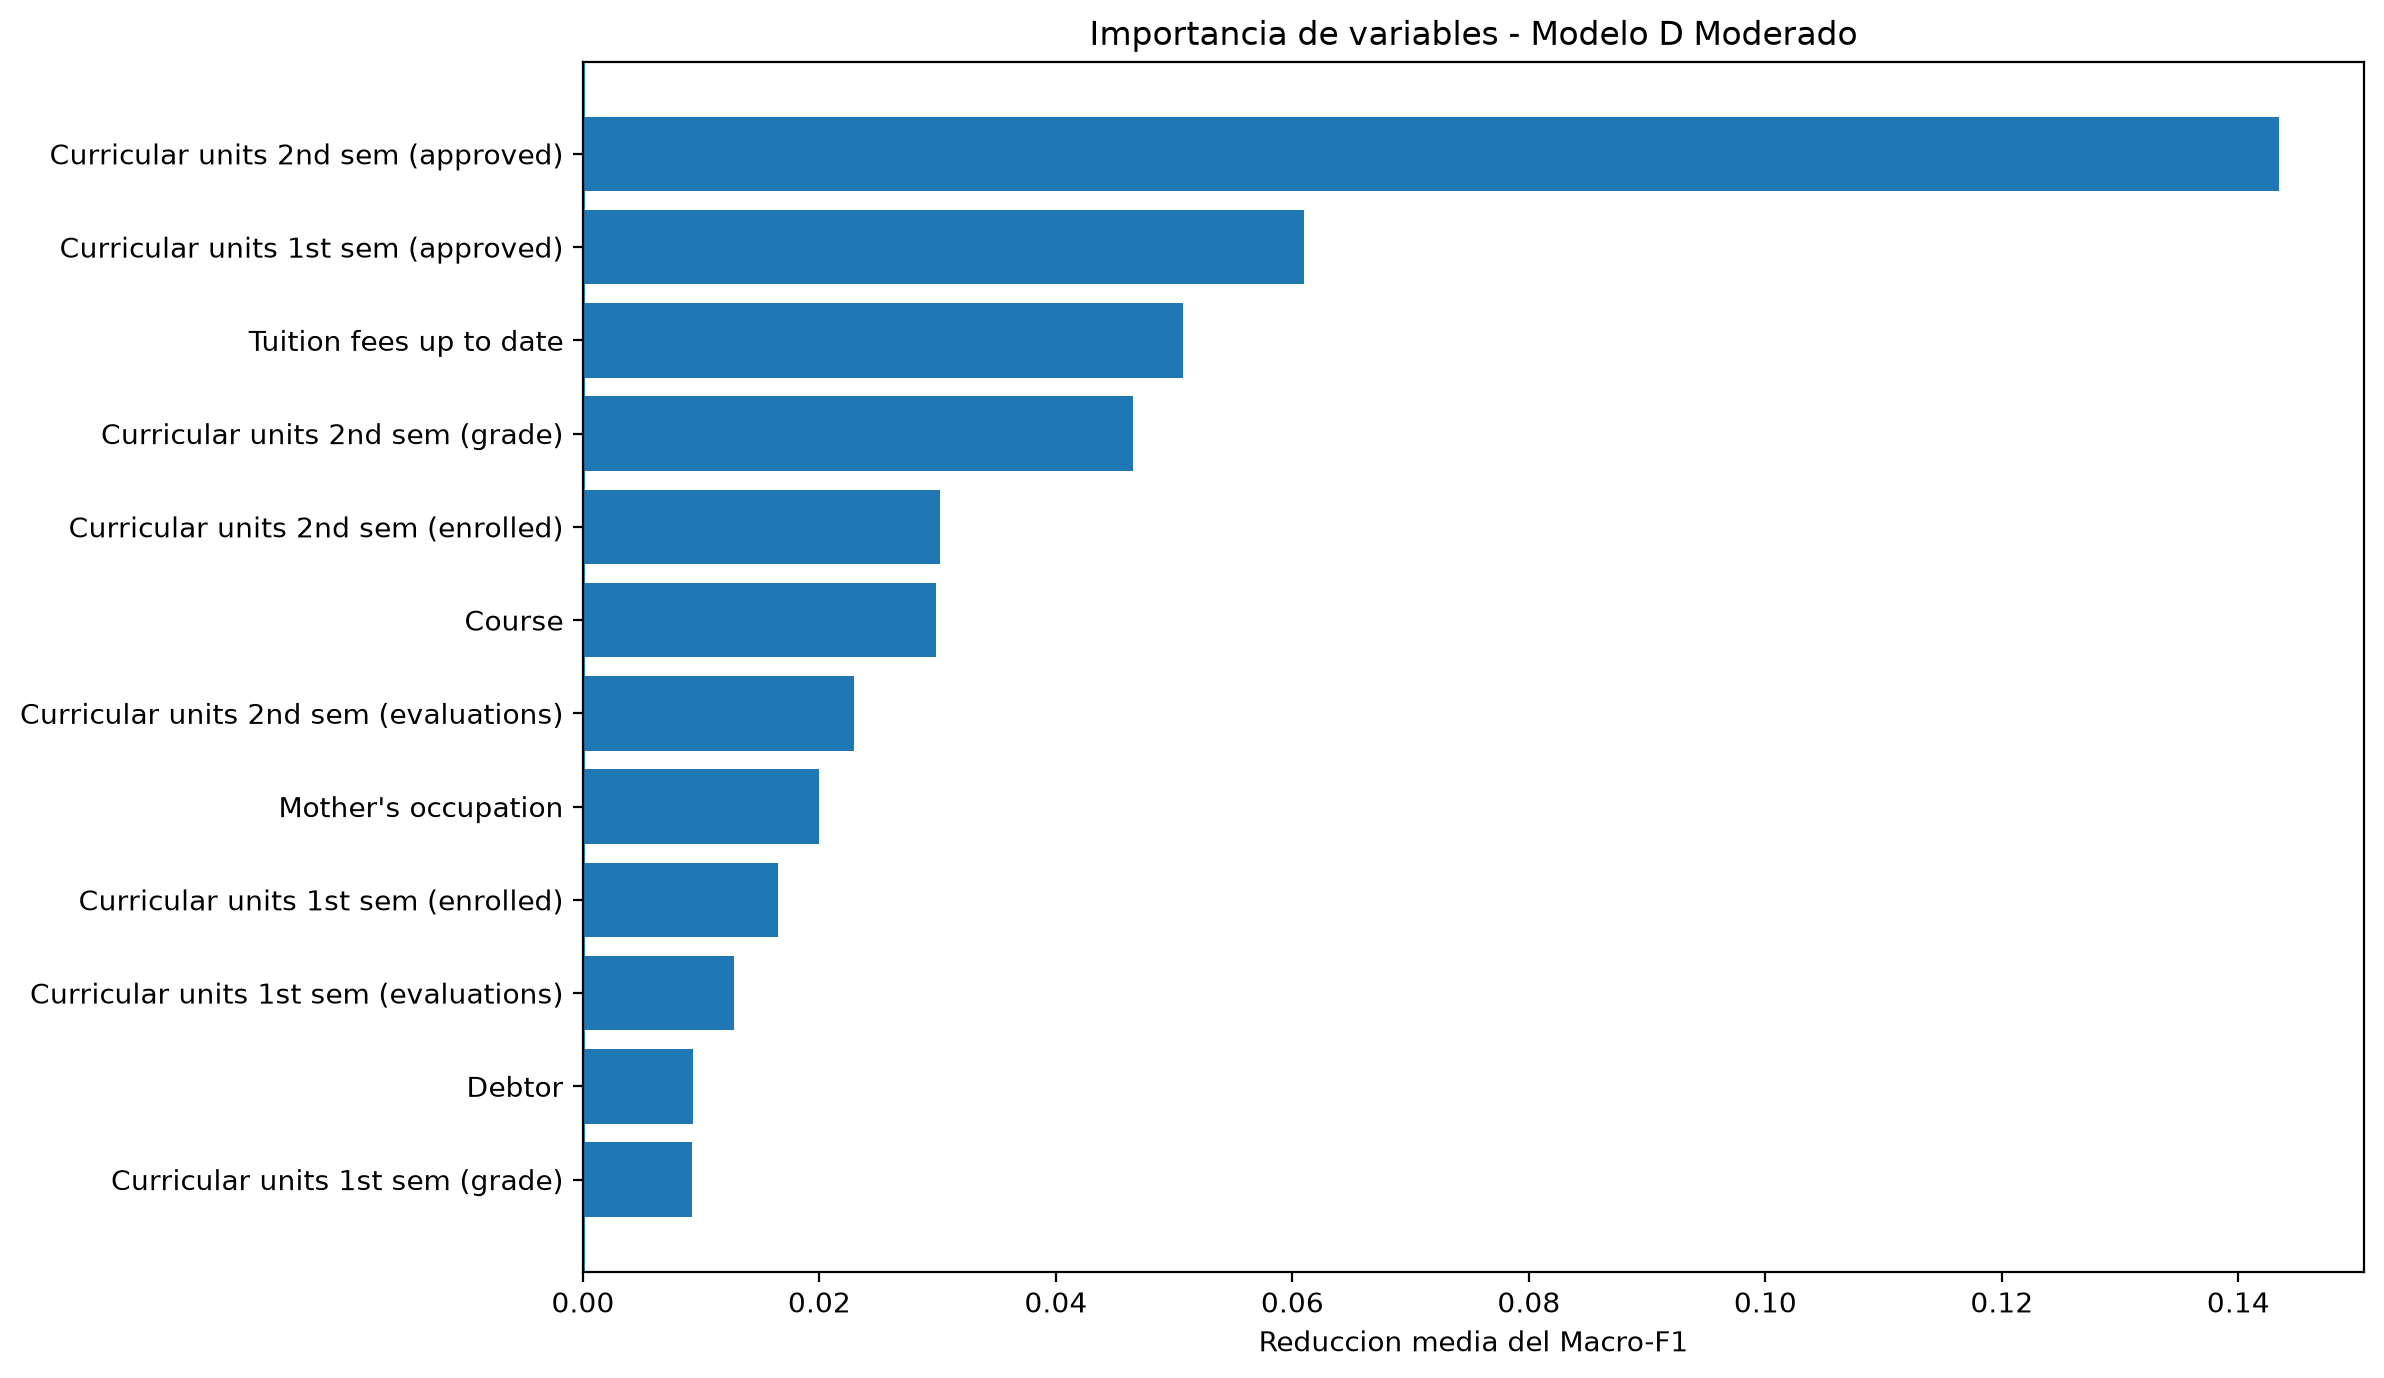
\includegraphics[width=0.98\linewidth]
{09_importancia_permutacion.png}
\caption{Importancia predictiva mediante permutación.}
\end{figure}

También destacaron las asignaturas aprobadas
en el primer semestre, las calificaciones,
la situación de matrícula y el programa académico.

La importancia de una variable no establece
una relación causal. Además, las variables
correlacionadas pueden compartir información
predictiva.

% ======================================
\section{Discusión}
% ======================================

Los resultados indican que el rendimiento
depende tanto de la información disponible
como de la estrategia de aprendizaje.

La incorporación de información semestral
mejoró considerablemente el rendimiento
respecto al escenario sin semestres.

Optuna mejoró varios resultados, aunque
no todos: en prueba, el modelo base del
escenario C superó a su versión optimizada.

El balanceo modificó la distribución de
errores. El modelo moderado mejoró el
reconocimiento de Enrolled, pero presentó
compensaciones en otras clases.

Por ello, la selección de un modelo no debe
reducirse únicamente a maximizar accuracy.

\subsection{Limitaciones}

\begin{itemize}
\item El dataset procede de un contexto institucional específico.
\item Solo se utilizó una división de desarrollo y prueba.
\item La clase Enrolled presentó dificultades de clasificación.
\item Algunas variables pueden tener disponibilidad temporal distinta.
\item No se realizó validación externa.
\item Los análisis de importancia no prueban causalidad.
\item No se evaluó el uso del modelo en decisiones institucionales reales.
\end{itemize}

% ======================================
\section{Conclusiones}
% ======================================

\begin{enumerate}
\item Se desarrolló un sistema de clasificación
multiclase con TensorFlow/Keras.

\item Se evaluaron cuatro escenarios y se
completaron 80 ensayos de optimización con Optuna.

\item La optimización mejoró varios escenarios,
pero no garantizó superioridad en prueba.

\item El balanceo moderado elevó el recall de
Enrolled frente al modelo D Optuna.

\item La mejora global del macro-F1 no fue
concluyente según el intervalo bootstrap.

\item El rendimiento académico del segundo semestre
destacó como fuente importante de información predictiva.

\item El estudio confirma la relevancia de
la evaluación por clase, la reproducibilidad
y el análisis crítico de resultados.
\end{enumerate}

% ======================================
\section{Respuestas a la actividad}
% ======================================

\subsection*{1. Método de búsqueda}

Se utilizó Optuna con TPESampler, un método de
optimización secuencial de hiperparámetros.

\subsection*{2. Hiperparámetros}

Se optimizaron número de capas, neuronas,
Dropout, regularización L2, learning rate
y tamaño de lote.

\subsection*{3. Mejoras obtenidas}

El resultado dependió del escenario.
La mayor mejora de macro-F1 en validación
se observó en A, con aproximadamente
8,38 puntos porcentuales.

En prueba, la optimización no fue superior
en todos los escenarios.
El balanceo moderado aumentó el recall de
Enrolled en el escenario D.

\subsection*{4. Mejoras futuras}

Sería conveniente explorar validación cruzada,
calibración probabilística, funciones de pérdida
alternativas, modelos clásicos comparativos
y validación sobre otras instituciones.

% ======================================
\section{Reproducibilidad}
% ======================================

El repositorio del proyecto incluye scripts de
preprocesamiento, entrenamiento, optimización,
evaluación, interpretabilidad y auditoría.

Las versiones de dependencias están registradas
en \texttt{requirements-lock.txt}.

El notebook ejecutado presenta las tablas
y los resultados ya obtenidos.

La evaluación final no debe repetirse
para seleccionar nuevas configuraciones
basadas en sus métricas.

% ======================================
\section*{Repositorio de GitHub y reproducibilidad}
% ======================================
El codigo fuente, los cuadernos Jupyter, los modelos
entrenados, las metricas de evaluacion y los resultados
experimentales del Proyecto 9 se encuentran disponibles
en el repositorio publico de GitHub.

\begin{center}
    \href{
    https://github.com/alexroma1126-design/proyecto9-keras-optuna-desercion-academica
    }{\textbf{Consultar el Proyecto 9 en GitHub}}
\end{center}

% ======================================
\begin{thebibliography}{9}

\bibitem{uci697}
UCI Machine Learning Repository.
\emph{Predict Students' Dropout and Academic Success}.
\url{https://archive.ics.uci.edu/dataset/697/predict+students+dropout+and+academic+success}

\bibitem{keras}
Keras.
\emph{Keras documentation}.
\url{https://keras.io/}

\bibitem{optuna}
Optuna.
\emph{Optuna documentation}.
\url{https://optuna.readthedocs.io/}

\bibitem{sklearn}
Scikit-learn.
\emph{User Guide}.
\url{https://scikit-learn.org/stable/user_guide.html}

\end{thebibliography}

\end{document}
